\setlength{\columnsep}{3pt}
\begin{flushleft}
	\bigskip
	
	\textbf{Exception Handling} allows you to separate error-handling code from normal code.
	
	\begin{figure}[h!]
		\centering
		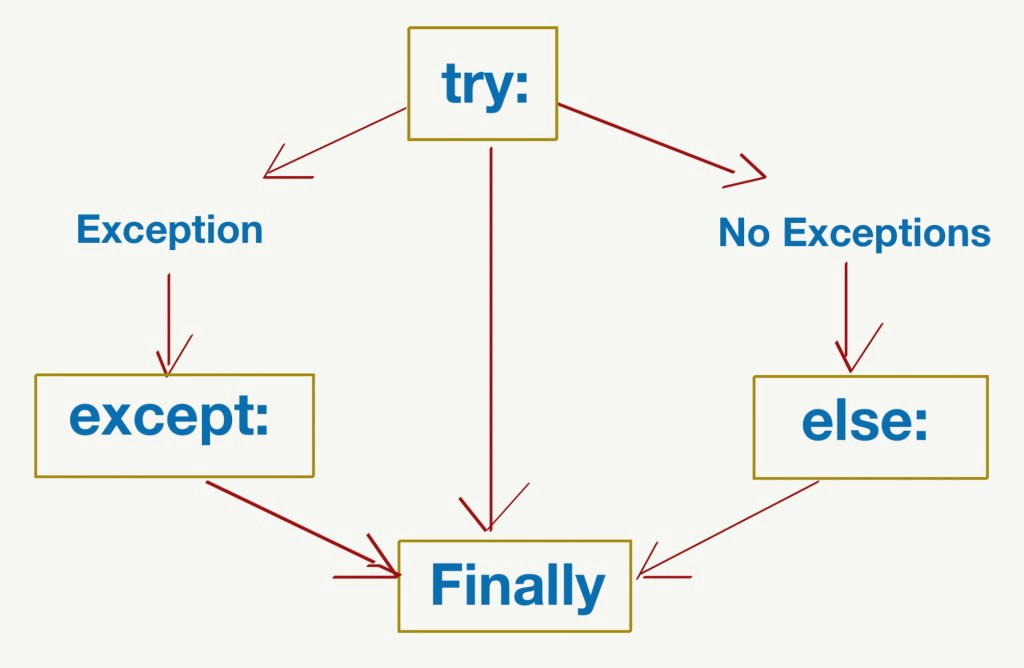
\includegraphics[scale=0.3]{content/chapter9/images/except.jpeg}
	\end{figure}
	
	\begin{itemize}
		\item \textbf{try}: Code block in which you expect an error to occur.
		\bigskip
		\item \textbf{except}: Define the action to be taken as per exception.
		\bigskip
		\item \textbf{else}: This block is executed if no exception is hit.
		\bigskip
		\item \textbf{finally}: This block of code will \textbf{always} be executed regardless of exception.	
	\end{itemize}

	\begin{tcolorbox}[breakable,notitle,boxrule=1pt,colback=pink,colframe=pink]
		\color{black}
		\fontdimen2\font=8pt
		Syntax: 
		\newline
		try: \newline
		\hphantom{} \hphantom{} statement \newline
		except EXCEPTION\_NAME: \newline
		\hphantom{} \hphantom{} statement \newline
		else: \newline
		\hphantom{} \hphantom{} statement \newline
		finally: \newline
		\hphantom{} \hphantom{} statement
		\fontdimen2\font=4pt
	\end{tcolorbox}
	
	\newpage
	
	\textbf{Example:}
	\begin{itemize}
		\item Generic exception example:
		\begin{tcolorbox}[breakable,notitle,boxrule=-0pt,colback=code,colframe=code]
			\color{white}
			\fontdimen2\font=8pt
			try: \newline
			\hphantom{} \hphantom{} import pandas \newline
			\hphantom{} \hphantom{} print("Code moving forward...") \newline
			except: \newline
			\hphantom{} \hphantom{} print('Oops something went wrong!') \newline
			else: \newline
			\hphantom{} \hphantom{} print('Code without exception')
			\fontdimen2\font=4pt
		\end{tcolorbox}
		
		Output: To hit the exception, make sure you uninstall "pandas" using command - "pip uninstall pandas"
	
		\begin{tcolorbox}[breakable,notitle,boxrule=-0pt,colback=error,colframe=error]
			\color{black}
			Oops something went wrong!
			\fontdimen2\font=4pt
		\end{tcolorbox}		


		\bigskip
		
		\item Catching specific exception example:
		\begin{tcolorbox}[breakable,notitle,boxrule=-0pt,colback=code,colframe=code]
			\color{white}
			\fontdimen2\font=8pt
			try: \newline
			\hphantom{} \hphantom{} import pandas \newline
			\hphantom{} \hphantom{} print("Code moving forward...") \newline
			except ImportError: \newline			
			\hphantom{} \hphantom{} print("Please execute: pip install pandas") \newline
			except: \newline
			\hphantom{} \hphantom{} print('Oops something went wrong!') \newline
			else: \newline
			\hphantom{} \hphantom{} print('Code without exception')
			\fontdimen2\font=4pt
		\end{tcolorbox}
		
		Output:
		\begin{tcolorbox}[breakable,notitle,boxrule=-0pt,colback=error,colframe=error]
			\color{black}
			Please execute:  \newline
			pip install pandas
			\fontdimen2\font=4pt
		\end{tcolorbox}		
	
		\newpage
		
		\item Catching specific exception example:
		\begin{tcolorbox}[breakable,notitle,boxrule=-0pt,colback=code,colframe=code]
			\color{white}
			\fontdimen2\font=8pt
			try: \newline
			\hphantom{} \hphantom{} import pandas \newline
			\hphantom{} \hphantom{} print("Code moving forward...") \newline
		    \hphantom{} \hphantom{} a=int(input("Enter number1: ")) \newline
			\hphantom{} \hphantom{} b=int(input("Enter number2: ")) \newline
			\hphantom{} \hphantom{} ans=a/b \newline
			\hphantom{} \hphantom{} print(f'{a}/{b}: {ans}') \newline
			except ImportError: \newline
			\hphantom{} \hphantom{} print("Please execute: pip install pandas") \newline
			except ZeroDivisionError: \newline
			\hphantom{} \hphantom{} print("You cannot divide a number by zero.") \newline
			except: \newline
			\hphantom{} \hphantom{} print('Oops something went wrong!') \newline
			else: \newline
			\hphantom{} \hphantom{} print('Code without exception')
			\fontdimen2\font=4pt
		\end{tcolorbox}
		
		Output: 
		\begin{tcolorbox}[breakable,notitle,boxrule=-0pt,colback=error,colframe=error]
			\color{black}
			Code moving forward...
			Enter number1: 45
			Enter number2: 0
			You cannot divide a number by zero.
			\fontdimen2\font=4pt
		\end{tcolorbox}		
	
		\newpage

		\item Finally block example:
		\begin{tcolorbox}[breakable,notitle,boxrule=-0pt,colback=code,colframe=code]
			\color{white}
			\fontdimen2\font=8pt
			file = open('test.txt', 'w')
			\newline
			try: \newline
			\hphantom{} \hphantom{} file.write("Testing.") \newline
			\hphantom{} \hphantom{} print("Writing to file.") \newline
			except IOError: \newline
			print("Could not write to file.") \newline
			else: \newline
			print("Write successful.") \newline
			finally: \newline
			file.close() \newline
			print("File closed.")
			\fontdimen2\font=4pt
		\end{tcolorbox}
		
		Output: 
		\begin{tcolorbox}[breakable,notitle,boxrule=-0pt,colback=error,colframe=error]
			\color{black}
			Code moving forward...
			Enter number1: 45
			Enter number2: 0
			You cannot divide a number by zero.
			\fontdimen2\font=4pt
		\end{tcolorbox}		
											
	
	\end{itemize}
	
\end{flushleft}

\newpage

